\documentclass[journal]{vgtc}                % final (journal style)
%\documentclass[review,journal]{vgtc}         % review (journal style)
%\documentclass[widereview]{vgtc}             % wide-spaced review
%\documentclass[preprint,journal]{vgtc}       % preprint (journal style)
%\documentclass[electronic,journal]{vgtc}     % electronic version, journal

%% Uncomment one of the lines above depending on where your paper is
%% in the conference process. ``review'' and ``widereview'' are for review
%% submission, ``preprint'' is for pre-publication, and the final version
%% doesn't use a specific qualifier. Further, ``electronic'' includes
%% hyperreferences for more convenient online viewing.

%% Please use one of the ``review'' options in combination with the
%% assigned online id (see below) ONLY if your paper uses a double blind
%% review process. Some conferences, like IEEE Vis and InfoVis, have NOT
%% in the past.

%% Please note that the use of figures other than the optional teaser is not permitted on the first page
%% of the journal version.  Figures should begin on the second page and be
%% in CMYK or Grey scale format, otherwise, color shifting may occur
%% during the printing process.  Papers submitted with figures other than the optional teaser on the
%% first page will be refused.

%% These three lines bring in essential packages: ``mathptmx'' for Type 1
%% typefaces, ``graphicx'' for inclusion of EPS figures. and ``times''
%% for proper handling of the times font family.

\usepackage{mathptmx}
\usepackage{graphicx}
\usepackage{times}
\usepackage{balance}
\usepackage[nooneline,hang,it,IT]{subfigure}

%% We encourage the use of mathptmx for consistent usage of times font
%% throughout the proceedings. However, if you encounter conflicts
%% with other math-related packages, you may want to disable it.

%% This turns references into clickable hyperlinks.
\usepackage[bookmarks,backref=true,linkcolor=black]{hyperref} %,colorlinks
\hypersetup{
  pdfauthor = {},
  pdftitle = {},
  pdfsubject = {},
  pdfkeywords = {},
  colorlinks=true,
  linkcolor= black,
  citecolor= black,
  pageanchor=true,
  urlcolor = black,
  plainpages = false,
  linktocpage
}

%% If you are submitting a paper to a conference for review with a double
%% blind reviewing process, please replace the value ``0'' below with your
%% OnlineID. Otherwise, you may safely leave it at ``0''.
\onlineid{0}

%% declare the category of your paper, only shown in review mode
\vgtccategory{Research}

%% allow for this line if you want the electronic option to work properly
\vgtcinsertpkg

%% In preprint mode you may define your own headline.
%\preprinttext{To appear in an IEEE VGTC sponsored conference.}

%% Paper title.

\title{AiPoker - Implementation of a Poker Agent}

%% This is how authors are specified in the journal style

%% indicate IEEE Member or Student Member in form indicated below
\author{John Holl\'en, Robin Berntsson, Simon Bergst\"om}
\authorfooter{
%% insert punctuation at end of each item
\item
 John Holl\'en, Robin Berntsson, Simon Bergstr\"om
}

%% Abstract section.
\abstract{ 
We will probably write this section the last thing we do. 
}
%% Keywords that describe your work. Will show as 'Index Terms' in journal
%% please capitalize first letter and insert punctuation after last keyword
\keywords{Monte Carlo Tree Search, Texas Hold'em}



%%%%%%%%%%%%%%%%%%%%%%%%%%%%%%%%%%%%%%%%%%%%%%%%%%%%%%%%%%%%%%%%
%%%%%%%%%%%%%%%%%%%%%% START OF THE PAPER %%%%%%%%%%%%%%%%%%%%%%
%%%%%%%%%%%%%%%%%%%%%%%%%%%%%%%%%%%%%%%%%%%%%%%%%%%%%%%%%%%%%%%%%

\begin{document}

%% The ``\maketitle'' command must be the first command after the
%% ``\begin{document}'' command. It prepares and prints the title block.

%% the only exception to this rule is the \firstsection command
\firstsection{Background}
\maketitle 
Texas Hold'em is a popular variant of poker, not just to play with friends but also online against other people for money. Poker belongs with the most difficult kind of card game to solve discretely since it is an stochastic game with imperfect information. The challenge of creating the best poker agent has attracted a lot of people and is a popular subject in AI development.

The theory behind Monte Carlo search trees will be studied within this project and tested as a part of the logic that will determine the actions of the poker agent. Smaller algorithms to improve the logic for the AI will be tested and implemented in combination of the Monte Carlo Search Tree to create the best possible poker agent.

\section{Theory}
\subsection{Characteristics of a Poker Player}
Like previously described poker is a stochastic game, that makes it very hard to control and to define what a good poker player is. A good poker player does not always need to be the one who is a winning player. But in this project a aim has been set to try to create a poker agent who wants to win and will not take too much risk when playing. But to not make the agent to predictable the agent shall randomly switch behavior between aggressive and passive playing. 

\section{Method}
\subsection{Basic Game Engine}
In order to even begin implementing an AI, the core poker game had to be implemented first. For simplicity the game implemented in this study is a two player game where a human player faces a computer AI. The player who starts is chosen at random when the game is started. The player that starts then puts one dollar in to the pot. The other player puts two dollars in the pot. Then the game is turn based like ordinary Texas Hold?em, the players can bet, check, call, raise and fold. And after each betting round cards are dealt to the table and the players combine the cards on hand with the cards on the table in order to get the strongest hand possible. 

To be able to test the game engine the computer was first set to do moves completely  at random. When all this was done the implementation of the AI could start.

\subsection{AI - techniques}
\subsubsection{Monte Carlo Tree Search}
Monte Carlo Tree Search (MCTS) is just like an algorithm like minimax based on a tree structure. By simulating a number of different outcomes a search tree is built based on the outcome of the simulation. More specifically the algorithm is made in four different stages which are repeated numerous times when the algorithm is being run. 

MCTS only starts with the root node of the tree and incrementally build the tree by repeating the following 4 steps. One of the pros with MCTS is that it is anytime, that is it will give a valid solution to the problem even if it is interrupted before it ends. However the quality of the solution is an estimate and is expected to be better the more time the MCTS keeps running. \\*\\*
\textbf{Selection}
\\*Selection is made by starting from the root node and then recursively select nodes until a leaf node is reached (this does not have to be a leaf of the game tree). To determine which node is the optimal one, the following upper bounds confidence formula is used: 

\begin{equation} \label{eq:upperconfidence}
	v_{i} + C \cdot \sqrt{\frac{\ln N}{n_{i}}}
\end{equation}

\section{Result}


\section{Conclusion}

\begin{figure}[here]
  \begin{center}
    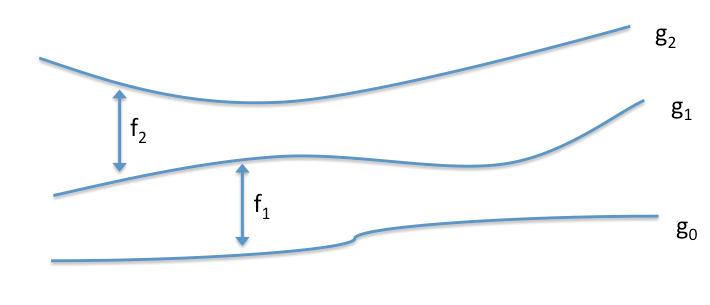
\includegraphics[scale=0.35]{img/stream1.png}
    \caption{\label{fig:streamexplanation}En bild for att se hur man lagger till bilder.}
  \end{center}
\end{figure}


\begin{thebibliography}{9}

\bibitem{byron}
  Byron L., Wattenberg M.
  \emph{Stacked graphs - Geometry \& Aesthetics}.
  IEEE Transactions on Visualization and Computer Graphics archive
Volume 14 Issue 6,
Pages 1245-1252. IEEE Educational Activities Department Piscataway, NJ, USA
ISSN: 1077-2626.
  2008.

\bibitem{reynolds}
  Reynolds A. P., Richards G., Rayward-Smith V. J.
  \emph{The Application of K-medoids and PAM to the Clustering of Rules}.
  In: Intelligent Data Engineering and Automated Learning - IDEAL 2004. Lecture Notes in Computer Science, 3177 . Springer-Verlag, pp. 173-178. ISBN 978-3-540-22881-3,
  2004.

\end{thebibliography}

\end{document}
